\documentclass{beamer}
\usetheme{AnnArbor}
\usecolortheme{beaver}
\usepackage{tikz}
\usepackage{color}
\usepackage{listings}

\lstset{language=Java,
  basicstyle=\footnotesize\ttfamily,
  keywordstyle=\footnotesize\color{blue}\ttfamily,
  commentstyle=\footnotesize\color{gray}\ttfamily,
}

\definecolor{darkred}{rgb}{0.8,0,0}

\setbeamercolor{title}{fg=white,bg=darkred!80!black}
\setbeamercolor{frametitle}{fg=darkred!80!black,bg=white}
%\setbeamercolor{section in head/foot}{fg=green,bg=yellow}
%\setbeamercolor{subsection in head/foot}{bg=white}
\begin{document}
\title{Advanced Java Debugging}   
\author{Andrej Podhradsky}
\date{February 8, 2016} 
%\logo{\includegraphics[height=1cm]{reddeer_logo.png}\vspace{220pt}}

\addtobeamertemplate{title page}{\center{DevConf 2016}}{}

%\addtobeamertemplate{frametitle}{}{
%\begin{tikzpicture}[remember picture,overlay]
%\node[anchor=north east,yshift=-8pt] at (current page.north east) {DevConf 2016};
%\end{tikzpicture}}

\frame{\titlepage} 

% \frame{\frametitle{Table of contents}\tableofcontents} 

\section{Motivation}

\subsection{What is debugging}
\begin{frame}[fragile]
\frametitle{What is debugging}
\begin{itemize}
\item process of finding and fixing bugs
\item usually time consuming
\item how would you debug this? (npe at line 3)
\vspace{0.2cm}
\begin{lstlisting}[numbers=left]
public User findUser(String nickname) {
  for (User user : this.users) {
    if (user.getNickname().equals(nickname)) {
      return user;
    }
  }
  return null;
}
\end{lstlisting}
\end{itemize}
\end{frame}


\subsection{First debug}
\begin{frame}[fragile]
\frametitle{Using sysout}
\begin{itemize}
\item there are 2 possibilities for npe
\vspace{0.2cm}
\begin{lstlisting}[numbers=left]
public User findUser(String nickname) {
  for (User user : this.users) {
    System.out.println("user=" + user);
    System.out.println("nickname=" + user.getNickname());
    if (user.getNickname().equals(nickname)) {
      return user;
    }
  }
  return null;
}
\end{lstlisting}
\end{itemize}
\end{frame}

\section{Prepare your environment}

\subsection{Prepare your environment}
\begin{frame}[fragile]
\frametitle{Prepare your environment}
\begin{itemize}
\item JDK 6+
  \begin{lstlisting}
    java -version
  \end{lstlisting}
\item Maven 3.0.5+
  \begin{lstlisting}
    mvn -v
  \end{lstlisting}
\item Eclipse IDE for Java (or JavaEE) Developers
  \begin{lstlisting}
    eclipse -data workspace
  \end{lstlisting}
\item FriendBook
  \begin{lstlisting}
    see next slides
  \end{lstlisting}
\end{itemize}
\end{frame}

\subsection{FriendBook}
\begin{frame}[fragile]
\frametitle{FriendBook}
\begin{center}
  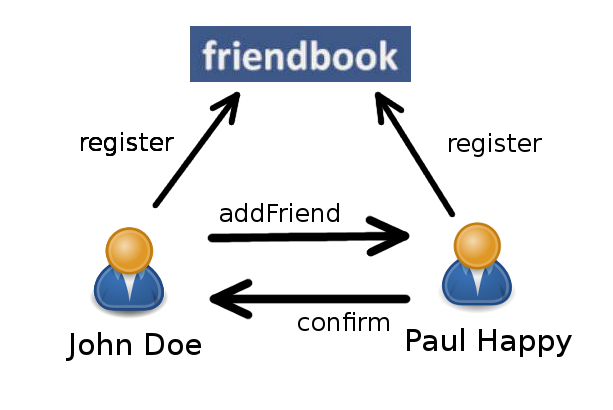
\includegraphics[width=11cm]{friendbook.png}
\end{center}  
\end{frame}


\section{Debugging}

\subsection{Breakpoints and variables}
\begin{frame}[fragile]
\frametitle{Breakpoints and variables}
\begin{itemize}
\item in a code
\item on an attribute
\item on a method
\item on an exception
\item view of variables
\end{itemize}
\end{frame}

\subsection{Conditional breakpoints}
\begin{frame}[fragile]
\frametitle{Conditional breakpoints}
\end{frame}

\subsection{Breakpoints and variables}
\begin{frame}[fragile]
\frametitle{Breakpoints and variables}
\end{frame}

\subsection{Display and watch the code}
\begin{frame}[fragile]
\frametitle{Display and watch the code}
\end{frame}

\subsection{Repeat the code}
\begin{frame}[fragile]
\frametitle{Repeat the code}
\begin{itemize}
\item repeat vs go back
\item you can jump only to a place in stack trace
\item (the stack of functions that were called up to that point)
\end{itemize}
\begin{lstlisting}
Exception in thread "main" java.lang.RuntimeException
    at test.stack.trace.SomeClass.methodC(SomeClass.java:18)
    at test.stack.trace.SomeClass.methodB(SomeClass.java:13)
    at test.stack.trace.SomeClass.methodA(SomeClass.java:9)
    at test.stack.trace.SomeClass.main(SomeClass.java:27)
\end{lstlisting}
\end{frame}

\subsection{Remote debugging}
\begin{frame}[fragile]
\frametitle{Remote debugging}
\end{frame}

\section{Learning Materials}
\begin{frame}[fragile]
\frametitle{Learning Materials}
\begin{itemize}
\item Effective Java Debugging with Eclipse\\\url{http://eclipsesource.com/blogs/2013/01/08/effective-java-debugging-with-eclipse}
\item Java Debugging with Eclipse - Tutorial\\url{http://www.vogella.com/tutorials/EclipseDebugging/article.html}
\end{itemize}
\end{frame}

\end{document}
